\documentclass[10pt]{article}
\usepackage{latexsym}
\usepackage{natbib}
\usepackage{graphicx}
\usepackage{subfigure}
\usepackage{listings}
\usepackage{algorithm}
\usepackage{algpseudocode}

\title{Homework 1: N-gram Language Models}
\author{Yu Feng}
\date{2-16-2015}

\begin{document}
\maketitle

\section{Introduction}
In this homework, my task is to produce both a ``backward" bigram model and a bidirectional model based on the sample code of a normal bigram model. 
 
\section{Algorithm}\label{sec:alg}

\subsection{Backward Bigram Model}

The algorithm for the backward bigram model is almost identical to the normal bigram model except for the model direction. So what I need to do is to swap the model direction for both the training and testing data and then invoke the original corresponding functions. 


\subsection{Bidirectional Bigram Model}

Here are the steps to build the bidirectional bigram model:

Step 1: Create an instance of the bidirectional model which has references to the instances of the bigram model and the backward bigram model;

Step 2: Train each model separately by invoking its own training method using the given data;

Step 3: When determining the probability of each word($\alpha_i$) using the bidirectional model, linearly interpolate the predicted results of the bigram model and the backward bigram model based on the following equation:
\[
  \alpha_{i} = log(\lambda_{1} * \beta_{i} + \lambda_{2} * \gamma_{i})
\] 
Here, $\beta_{i}$ and $\gamma_{i}$ are the probability predicted by the bigram model and the backward bigram model, respectively. $\lambda_{1}$, $\lambda_{2}$ are their corresponding weight. I weight them equally in the experiment. 

Step 4: The probability for the entire sentence will be the sum of all its words:
\[
   \Psi = \sum_{i=1}^{n}{ \alpha_{i}}
\]
 where $n$ is the number of words in current sentence.
\section{Experiments}\label{sec:exp}

I implemented the algorithms described in section~\ref{sec:alg} and tested them on the \emph{atis}, \emph{wsj} and \emph{brown} corpora. In this section I will study the experimental results from different aspects.

\textbf{A quick glance}: In my first step, I ran three models on the above data with the default setting from class: using 10\% sentences as the testing data and splitting the weights of the Bigram model and Backward model evenly in the Bidirectional model. Table~\ref{table:train} and Table~\ref{table:test} shows the overall results for word perplexity. The results show that Bidirectional model outperforms other models in all benchmark and it's hard to tell whether the Bigram model is better than the Backward model or the other way around: Backward model is slightly better in \emph{wsj} and \emph{brown} but worse in \emph{atis}.

\textbf{Fractions of sentences in testing set}: In the second step, I re-ran the entire experiment by setting the fraction of testing data from 0.1 to 0.9. For the Bidirectional model, the weights of the Bigram model and Backward model are still split evenly. The goal of this experiment is to evaluate the effectiveness of the above three model in diverse data set.

Figure~\ref{fig:test1}, figure~\ref{fig:test2} and figure~\ref{fig:test3} show the results of \emph{atis}, \emph{wsj} and \emph{brown} respectively. With those mass data, I began to get the big picture of those three models:

\begin{itemize}
  \item Bidirectional model still outperforms other two models in all different settings;
  \item For the comparison between the Bigram model and the Backward model, their word perplexity are very closed to each other comparing their differences with the Bidirectional model; Backward model is slightly better in \emph{wsj} and \emph{brown} but worse in \emph{atis};
  \item If we look at the results closely, it's very interesting that all of those three models reach their optimal value(lowest word perplexity) while using 90\% of testing data.(The Bidirectional model in figure~\ref{fig:test2} is the only exception.) This is a bit counterintuitive to me: the testing result is supposed to be better when we have more training data.
\end{itemize}

\textbf{Weights of Bigram model in the Bidirectional Model}: In the final step, I evaluated the performance of the Bidirectional model by the following: I fixed the fraction of test data(10\%) and changed the weight of the Bigram model from 0.1 to 0.9. Then I re-ran the Bidirectional model on all the three data set.

Figure~\ref{fig:bi} shows the result of the experiment. For the data set in \emph{wsj} and \emph{brown}, the Bidirectional reaches it optimal solution when the weight is 0.5. On the other hand, \emph{atis} gets the optimal value with the weight of 0.9.



\begin{table}
\begin{center}
\begin{tabular}{|l|l|l|l|l|}  \hline
POS Data    & Bigram & Backward & Bidirectional \\ \hline
atis        & 10.592 & 11.636 & 7.235  \\ \hline
wsj         & 88.890 & 86.660 & 46.514  \\  \hline
brown       & 113.360 & 110.783 & 61.469  \\  \hline
\end{tabular}
\caption{\small Comparison of Word Perplexity among three models on the training data from the atis, wsj and brown corpora.}\label{table:train}
\end{center}
\end{table}

\begin{table}
\begin{center}
\begin{tabular}{|l|l|l|l|l|}  \hline
POS Data    & Bigram & Backward & Bidirectional \\ \hline
atis        & 24.054 & 27.161 & 12.700  \\ \hline
wsj         & 275.118 & 266.352 & 126.113  \\  \hline
brown       & 310.667 & 299.686 & 167.487  \\  \hline
\end{tabular}
\caption{\small Comparison of Word Perplexity among three models on the testing data from the atis, wsj and brown corpora.}\label{table:test}
\end{center}
\end{table}



\begin{figure}
\centering
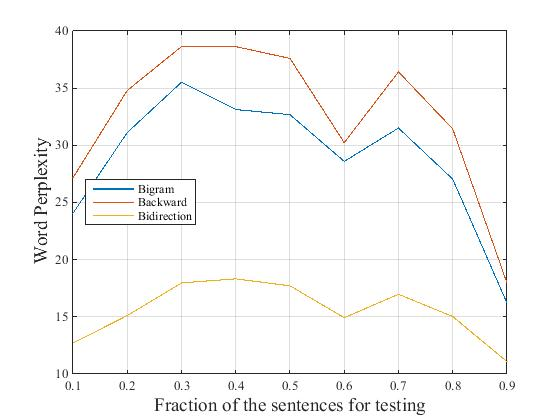
\includegraphics[scale=0.5]{test_atis.jpg}
\caption{Evaluation on different fraction of testing set for atis}\label{fig:test1}
\end{figure}

\begin{figure}
\centering
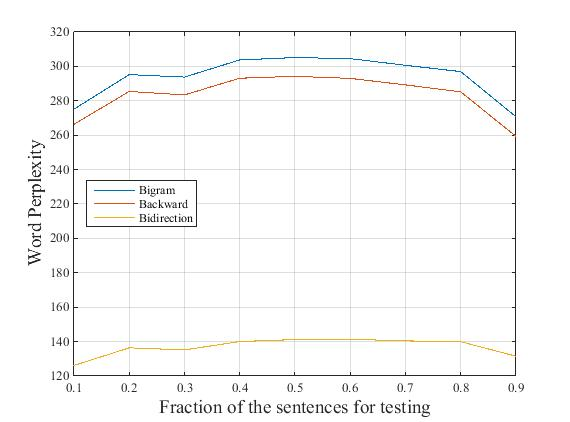
\includegraphics[scale=0.5]{test_wsj.jpg}
\caption{Evaluation on different fraction of testing set for wsj}\label{fig:test2}
\end{figure}

\begin{figure}
\centering
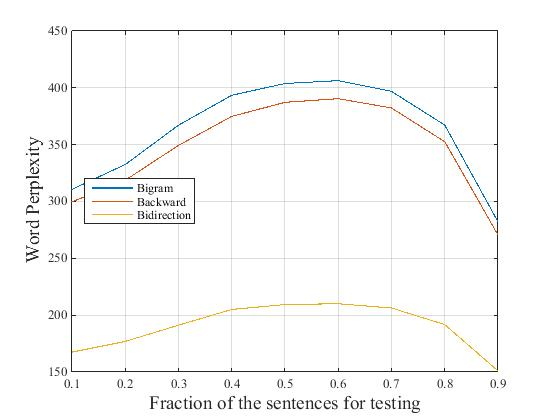
\includegraphics[scale=0.5]{test_brown.jpg}
\caption{Evaluation on different fraction of testing set for brown}\label{fig:test3}
\end{figure}

\begin{figure}
\centering
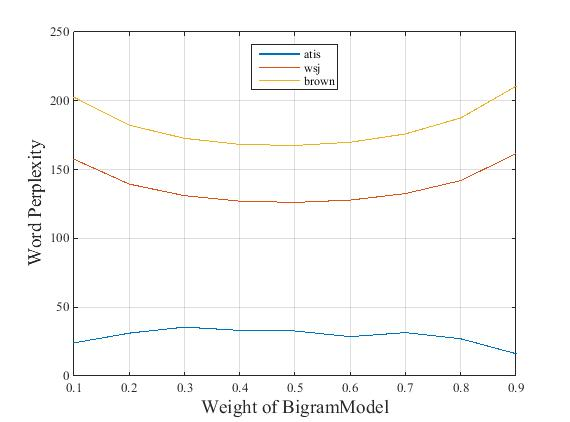
\includegraphics[scale=0.5]{bidirect.jpg}
\caption{Evaluation on different weight of bigramModel}\label{fig:bi}
\end{figure}
\section{Conclusion}

To conclude, based on the results in section~\ref{sec:exp}, the Bidirectional model strictly outperforms other models in all three benchmarks in terms of the word perplexity. This is reasonable because the bidirectional algorithm is taking advantage of the knowledge from both sides. When predicting each token, the bidirectional model has contexts from both forward and backward which leads to a high prediction rate. On the other hand, for the backward model and the normal Bigram model, we can't tell which one is better. Given a corpora with large size, the results in \emph{wsj} and \emph{brown} show that the word perplexity of those two models are quite closed to each other. One reason could be, in natural language, there exists both forward and backward regularity.

Regarding the word perplexity in the bidirectional model, figure~\ref{fig:bi} shows that it could reach an optimal value when the weight of backward and forward models are split evenly.

One interesting observation is, increasing the fraction of training data will not necessarily lead to a higher word perplexity.



\end{document}
